\documentclass{article}
\usepackage{mainPoly}

\title{Dérivation globale}
\author{Premières Spécialité Mathématiques}
\date{}

\begin{document}
\maketitle
\section{Fonction dérivée}
\begin{remark}
On rappelle qu'une fonction $f$ définie sur un intervalle $I$ est dite \textbf{dérivable en $a \in I$} si et seulement si le taux de variation
\begin{equation*}
T_a(h) = \dfrac{f(a+h)-f(a)}{h}
\end{equation*}
admet une limite finie quand $h$ tend vers $0$. La valeur de cette limite $\lim_{h \to 0} T_a(h)$ est alors appelé \textbf{nombre dérivé de $f$ en $a$} et est noté $f'(a)$.

En résumé, la notion de dérivation est un processus dépendant de $f$ qui à tout nombre $a$ associe, quand c'est possible, un autre nombre $f'(a)$. Il s'agit donc d'une \textbf{fonction}.
\end{remark}
\begin{tcolorbox}
\begin{definition}
Soit $f$ une fonction définie sur un intervalle $I$. On dit que $f$ est \textbf{dérivable sur $I$} si pour tout nombre $a \in I$, la fonction $f$ est dérivable en $a$. Dans ce cas, on pose $f'$ la fonction définie sur $I$ qui à tout $x \in I$ associe le nombre dérivé $f'(x)$.  
\end{definition}
\end{tcolorbox}
\begin{example}
Soit $\function{f}{\R}{\R}{x}{x^2}$.

\begin{enumquestions}
\item Après avoir vérifié que $f$ est dérivable en $-3$, calculer $f'(-3)$.

\emptybox{5cm}
\item La valeur $-3$ a-t-elle eu spécifiquement un impact dans votre démonstration ? \answersline
\item En reprenant votre démonstration pour calculer $f'(x)$, où $x$ est une indéterminée, en déduire que $f$ est dérivable sur $\R$.

\emptybox{5cm}
\end{enumquestions}
\end{example}
\newpage
\begin{tcolorbox}
\begin{proposition}
\hfill
\begin{enumerate}
\item Soit $c \in \R$. La fonction constante définie sur $\R$ $f : x \mapsto c$ est dérivable sur $\R$, et sa dérivée est $f' : x \mapsto 0$.
\item La fonction identité définie sur $\R$ par $f : x \mapsto x$ est dérivable sur $\R$, et sa dérivée est $f' : x \mapsto 1$.
\item La fonction carré définie sur $\R$ par $f : x \mapsto x^2$ est dérivable sur $\R$, et sa dérivée est $f' : x \mapsto 2x$.
\item La fonction puissance $n \in \N$ définie sur $\R$ par $f : x \mapsto x^n$ est déribale sur $\R$, et sa dérivée est $f' : x \mapsto nx^{n-1}$
\item La fonction inverse définie sur $]-\infty;0[\cup]0;+\infty[$ par $f : x \mapsto \dfrac{1}{x}$ est dérivable sur $]-\infty;0[\cup]0;+\infty[$, et sa dérivée est $f' : x \mapsto -\dfrac{1}{x^2}$.
\item La fonction racine carrée définie sur $[0;+\infty[$ par $f : x \mapsto \sqrt{x}$ est dérivable sur $]0;+\infty[$, et sa dérivée est $f' : x \mapsto \dfrac{1}{2\sqrt{x}}$.
\end{enumerate}
\end{proposition}
\end{tcolorbox}
\begin{remark}
\hfill
\begin{itemize}
\item Avant de dériver une fonction, il faut s'assurer qu'elle est bien dérivable.
\item La fonction racine carrée est dérivable sur $]0;+\infty[$ \textbf{(ouvert en 0)}, tandis qu'elle sur définie sur $[0;+\infty[$ \textbf{(fermé en 0)}. En effet, la fonction n'est pas dérivable en $0$.
\end{itemize}
\end{remark}
\begin{proof}
\hfill

\vspace*{0.2cm}
\emptybox{10cm}
\end{proof}
\newpage

\section{Opération algébriques}
\begin{tcolorbox}
\begin{proposition}
Soient $u$ et $v$ deux fonctions définies et dérivables sur un intervalle $I$ \textbf{ouvert}.
\begin{itemize}
\item La fonction somme de $u$ et $v$ définie sur $I$ par $s(x) = u(x) + v(x)$ est dérivable sur $I$, et sa dérivée vérifie, pour tout $x \in I$, $s'(x) = u'(x) + v'(x)$. $\left((u+v)' = u' + v'\right)$
\item La fonction produit de $u$ et $v$ définie sur $I$ par $p(x) = u(x) \times v(x)$ est dérivable sur $I$, et sa dérivée vérifie, pour tout $x \in I$, $p'(x) = u'(x)v(x) + u(x)v'(x)$. $\left((uv)' = u'v + uv'\right)$
\item En particulier, le produit $p$ d'une fonction $u$ définie sur $I$ par une constante $a \in \R$, définie par $p(x) = a \times u(x)$, est dérivable sur $I$, et sa dérivée vérifie, pour tout $x \in I$, $p'(x) = a u'(x)$.
\item Si la fonction $v$ ne s'annule pas sur l'intervalle $I$, alors la fonction inverse de $v$ définie sur $I$ par $i(x) = \dfrac{1}{v(x)}$ est dérivable sur $I$, et sa dérivée vérifie, pour tout $x \in I$, $i'(x) = -\dfrac{v'}{v^2(x)}$. $\left(\left(\dfrac{1}{v}\right)' = -\dfrac{v'}{v^2}\right)$
\item Si la fonction $v$ ne s'annule pas sur l'intervalle $I$, alors la fonction quotient de $u$ et de $v$ définie sur $I$ par $q(x) = \dfrac{u(x)}{v(x)}$ est dérivable sur $I$, et sa dérivée vérifie, pour tout $x \in I$, $q'(x) = \dfrac{u'(x)v(x) - u(x)v'(x)}{v^2(x)}$. $\left(\left(\dfrac{u}{v}\right)' = \dfrac{u'v - uv'}{v^2}\right)$
\end{itemize}
\end{proposition}
\end{tcolorbox}
\begin{example}
Soient $u$ et $v$ deux fonctions définies sur $\R_+^*$ par:
\begin{equation*}
\begin{cases}
u(x) = x^2 -5x& \text{ pour tout } x \in \R_+^*\\
v(x) = \sqrt{x} + 1& \text{ pour tout } x \in \R_+^*
\end{cases}
\end{equation*}
\begin{enumquestions}
\item Les fonctions $u$ et $v$ sont-elles dérivables sur $\R_+^*$ ? Donner l'expression de leur dérivée.

\vspace*{0.2cm}
\emptybox{6cm}
\item En déduire la dérivée de la somme, du produit et du quotient de $u$ et $v$.

\vspace*{0.2cm}
\emptybox{6cm}
\end{enumquestions}
\end{example}
\section{Composition de fonctions}
\begin{tcolorbox}
\begin{definition}
Soit $f$ une fonction définie sur un intervalle $I$. On pose aussi $a$ et $b$ deux nombres réels. Enfin, on pose $J$ l'intervalle des réels $x$ tels que $ax+b \in I$. 

Alors on appelle la fonction $g$ définie pour tout $x \in J$ par
\begin{equation*}
g(x) = f(ax+b)
\end{equation*}
la \textbf{fonction composée} de $f$ par la fonction $x \mapsto ax + b$.
\end{definition}
\end{tcolorbox}
\begin{proposition}
Soit $f$ une fonction définie et dérivable sur un intervalle $I$, $a$ et $b$ deux réels et $J$ l'intervalle des $x$ vérifiant $ax+b \in I$. Alors la fonction composée de $f$ par $x \mapsto ax + b$, c'est-à-dire la fonction définie pour tout $x \in J$ par $g(x) = f(ax+b)$ est dérivable sur $J$, et sa dérivée vaut pour tout $x \in J$,
\begin{equation*}
g'(x) = af'(ax+b)
\end{equation*}
\end{proposition}
\begin{example}
Soit la fonction $g$ définie sur un certain intervalle $J$ par la formule
\begin{equation*}
g(x) = \sqrt{3x - 2} \text{ pour tout } x \in J
\end{equation*}
\begin{enumquestions}
\item Identifier le plus grand intervalle \textbf{ouvert} $J$ sur lequel cette fonction est définie.

\vspace*{0.2cm}
\emptybox{2cm}
\item De quelles fonctions $g$ est-elle la composée ?

\vspace*{0.2cm}
\emptybox{2cm}
\item En déduire que $g$ est dérivable sur $J$, et calculer sa dérivée.

\vspace*{0.2cm}
\emptybox{4cm}
\end{enumquestions}
\end{example}
\newpage
\section{Variations de fonctions dérivables}
\begin{tcolorbox}
\begin{proposition}
Soit $f$ une fonction définie et dérivable sur un intervalle $I$.
\begin{itemize}
\item La fonction $f$ est \textbf{croissante} sur $I$ si et seulement si $f'$ est \textbf{positive} sur $I$.
\item La fonction $f$ est \textbf{décroissante} sur $I$ si et seulement si $f'$ est \textbf{négative} sur $I$.
\item La fonction $f$ est \textbf{constante} sur $I$ si et seulement si $f'$ est \textbf{nulle} sur $I$  
\end{itemize}        
\end{proposition}
\end{tcolorbox}
\begin{remark}
\begin{itemize}
\item Cela correspond à l'intuition grâce à laquelle la dérivée a été construite, c'est-à-dire que $f'(x)$ est la pente de la tangente à la courbe représentative de $f$ en le point $(x;f(x))$.
\item Ce sont des équivalences. Si la fonction est croissante, alors sa dérivée est positive. Si la dérivée d'une fonction est positive, alors cette fonction est croissante.
\end{itemize}
\end{remark}
\begin{example}
Soit $f : x \mapsto x^2 - 2x + 1$ définie sur $\R$.
\begin{enumquestions}
\item Donner l'expression de la dérivée de $f$. \answersline
\item Étudier le signe de $f'$ à l'aide d'un tableau de signe.
\begin{center}
\begin{tikzpicture}
\tkzTabInit{$x$/0.5, Signe de $f'$/2}{$-\infty$, $\cdots$, $+\infty$};
\end{tikzpicture}
\end{center}
\item En déduire le tableau de variations de $f$.
\begin{center}
\begin{tikzpicture}
\tkzTabInit{$x$/0.5, Variations de $f$/2}{$-\infty$, $\cdots$, $+\infty$};
\end{tikzpicture}
\end{center}
\end{enumquestions}
\end{example}
\newpage
\section{Extremums de fonctions dérivables}
\begin{tcolorbox}
\begin{definition}
Soit $f$ une fonction définie sur un intervalle $I$, et $a \in I$. On dit que $f$ atteint un \textbf{extremum local} en $a$ s'il existe un intervalle (non restreint à un point) $J$ tel que : $a \in J$; $J \subseteq I$ et la restriction de $f$ sur $J$ atteint un extremum en $a$.   
\end{definition}
\end{tcolorbox}
\begin{remark}
Autrement dit, $f(a)$ est un extremum local de $f$ sur $I$ si l'image de $a$ est supérieure ou inférieure à l'image de ses voisins \og proches \fg.
\end{remark}
\begin{example}
Soit $f$ une fonction définie sur $[-6;6]$ dont la courbe représentative $\mathcal{C}_f$ est représentée sur le repère suivant (en bas à gauche) :
\begin{center}
\hfill
\begin{tikzpicture}
\repereclassique{-3.25}{-3.25}{3.25}{3.25}{0.5};
\draw (-3,0) parabola bend (-1.5,2) (-0.5,0);
\draw (-0.5,0) parabola bend (1,-1) (1.5,0);
\draw (1.5,0) parabola bend (2,2.5) (3,1.5) node[below right] {$\mathcal{C}_f$};
\draw (-3,0) node {$\bullet$};
\draw (3,1.5) node {$\bullet$};
\end{tikzpicture}
\hfill
\begin{tikzpicture}
\repereclassique{-3.25}{-3.25}{3.25}{3.25}{0.5};
\draw (-3,0) parabola bend (-1.5,2) (-0.5,0);
\draw (-3,0) node {$\bullet$};
\draw (-0.5,0) node {$\bullet$};
\end{tikzpicture}
\hfill
\end{center}
\begin{enumquestions}
\item Quel est le maximum et le minimum de $f$ ? En quelles valeurs sont-elles atteintes ?
\item On a représenté sur le repère à droite la restriction de $f$ sur l'intervalle $[-6;-1]$. En déduire que en quel abscisse $f$ admet un extremum local.  
\end{enumquestions}
\emptybox{2cm}
\end{example}
\begin{tcolorbox}
\begin{proposition}
Soit $f$ une fonction définie et dérivable sur un intervalle \textbf{ouvert} $I$, et soit $a \in I$. Si $f$ atteint un extremum local en $a$, alors
\begin{equation*}
f'(a) = 0
\end{equation*} 
\end{proposition}
\end{tcolorbox}
\begin{remark}
\hfill
\begin{itemize}
\item \textbf{L'hypothèse d'intervalle ouvert est importante} : cette proposition devient fausse sinon. Par exemple, la fonction carrée $f \colon x \mapsto x^2$ restreinte sur $[1;2]$ admet un extremum en $1$, mais sa dérivée en $1$ est non-nulle.
\item \textbf{La réciproque de cette proposition est fausse} : ce n'est pas forcément parce que $f'(a) = 0$ que $f$ atteint un extremum local en $a$. Par exemple, si $f \colon x \mapsto x^3$ sur $\R$, on a bien $f'(0) = 0$, et pourtant $f(0) = 0$ n'est ni un minimum ou un maximum local.
\item Cette proposition donne néanmoins une liste des candidats envisageables pour lex extremums d'une fonction dérivable sur un intervalle $I$ : il suffit de chercher parmi les points $a$ tels que $f'(a) = 0$. C'est ce qu'on appelle une \textbf{condition nécessaire}.
\end{itemize}
\end{remark}
\end{document}